
\clearpage
\section{Konzept}\label{sec:Konzept}
Der Aufbau des digitalen Theremin ist sehr ähnlich wie das des Analogen, mit einigen Änderungen um es besser digital aufzubauen. Abbildung \ref{img:Blockschaltbild_digital} zeigt, dass der Lautstärke- und Tonhöhenoszillator nicht mehr einen Sinus sondern einen Rechteck generieren. Wir haben uns deshalb für diese Änderung entschieden, da es so einfacher ist das Signal in das FPGA einzulesen, da kein Analog-Digital-Wandler nötig ist. Weil der Referenzoszillator weiterhin einen Sinus generiert, ergibt die Mischung mit dem Rechteck auch Mischprodukte mit dessen Oberwellen. Da diese aber eine höhere Frequenz haben, ist eine spätere Filterung möglich.\\
Weiter sind die Referenzoszillatoren neu digital. Um nun einen Sinus zu generieren, haben wir uns entschieden den in Kapitel \ref{subsec:Cordic} behandelten Cordic Algorithmus zu verwenden. Dieser ist besser um verschiedene Frequenzen zu generieren als eine einfache Lookup-Table und bietet einen grösseren Lerngewinn. Diese Komponente stammt aus dem Projekt 5. \\
Der Mischer multipliziert den Sinus des Referenzoszillators mit dem Rechteck des analogen Oszillators. Auch diese Komponente stammt aus dem Projekt 5\\
Für das Tiefpassfilter haben wir uns entschieden mehrere CIC-Filter und ein FIR-Filter einzusetzen. Das CIC-Filter stammt ebenfalls aus dem Projekt 5. CIC-Filter haben den Vorteil, dass sie Ressourcensparender sind als äquivalente FIR-Filter.\\
Wie man sieht ist die Signalverarbeitung für den Lautstärkenverarbeitung bei diesem Aufbau gleich wie der Tonhöhenverarbeitung. Dies haben wir so entschieden, um dieselben Komponenten nochmals nutzen zu können.\\
Um das Audiosignal zu verstärken,benötigt der Verstärker die Frequenzinformation der Lautstärkenverarbeitung. Diese erhält er vom Block Frequenzmessung. Da die Frequenz des Lautstärkeoszillators bei Veränderung der Distanz zu der Antenne exponentiell ändert, ist keinerlei Umrechnung nötig um eine exponentielle Lautstärkeänderung zu erzielen.
Anschliessend konvertiert der Digital-Analog-Wandler das verstärkte Audiosignal und gibt es am Lautsprecher aus.\\
Wir entschieden zudem ein Nios II System einzusetzen um das Theremin zu bedienen und zu steuern. Dies hauptsächlich, um einen Einblick in den Nios II zu gewinnen und um eine Implementation der Steuerung zu vereinfachen. Für die Interagierung mit dem Theremin entschieden wir uns für ein Touch Display. Der Bedienungs \& Steuerungs Block (Nios System) wurde in Abbildung \ref{img:Blockschaltbild_digital} nicht mit anderen Komponenten verbunden um die Zeichnung übersichtlicher zu gestalten.

Über die Steuerung soll zudem eine automatische Kalibration des Theremins möglich sein. Diese soll die verschiedenen Oszillatoren so aufeinander abstimmen, dass eine Annäherung an die Antennen eine Erhöhung der Tonhöhe und Lautstärke bewirkt.

Es soll zudem möglich sein den in Kapitel \ref{sec:Einleitung} erwähnten Glissando-Effekt zu aktivieren und auf dem Display die Spielgenauigkeit anzuzeigen. Diese beiden Features werden über den Nios II und das Display gesteuert. Die Übergangszeit des Glissando-Effekt soll zudem einstellbar sein und es soll nebst der normalen Tonleiter auch die pentatonische Tonleiter spielbar sein.

\begin{figure}[h]
	\centering
	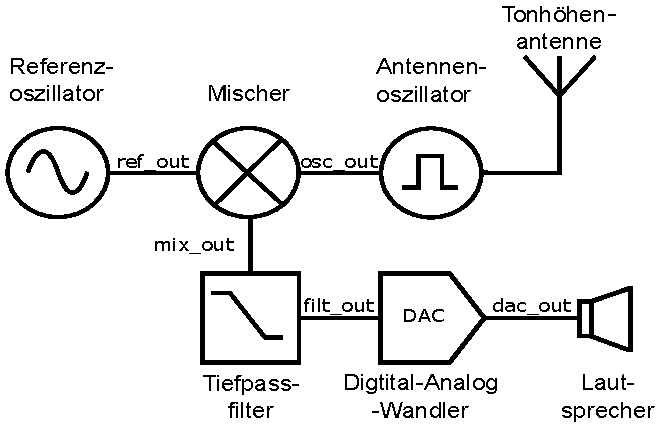
\includegraphics[width=\textwidth]{Blockschaltbild_digital.pdf}
	\caption{Blockschaltbild des digitalen Theremins}
	\label{img:Blockschaltbild_digital}
\end{figure}